% Options for packages loaded elsewhere
\PassOptionsToPackage{unicode}{hyperref}
\PassOptionsToPackage{hyphens}{url}
%
\documentclass[
]{article}
\usepackage{amsmath,amssymb}
\usepackage{iftex}
\ifPDFTeX
  \usepackage[T1]{fontenc}
  \usepackage[utf8]{inputenc}
  \usepackage{textcomp} % provide euro and other symbols
\else % if luatex or xetex
  \usepackage{unicode-math} % this also loads fontspec
  \defaultfontfeatures{Scale=MatchLowercase}
  \defaultfontfeatures[\rmfamily]{Ligatures=TeX,Scale=1}
\fi
\usepackage{lmodern}
\ifPDFTeX\else
  % xetex/luatex font selection
\fi
% Use upquote if available, for straight quotes in verbatim environments
\IfFileExists{upquote.sty}{\usepackage{upquote}}{}
\IfFileExists{microtype.sty}{% use microtype if available
  \usepackage[]{microtype}
  \UseMicrotypeSet[protrusion]{basicmath} % disable protrusion for tt fonts
}{}
\makeatletter
\@ifundefined{KOMAClassName}{% if non-KOMA class
  \IfFileExists{parskip.sty}{%
    \usepackage{parskip}
  }{% else
    \setlength{\parindent}{0pt}
    \setlength{\parskip}{6pt plus 2pt minus 1pt}}
}{% if KOMA class
  \KOMAoptions{parskip=half}}
\makeatother
\usepackage{xcolor}
\usepackage[margin=1in]{geometry}
\usepackage{color}
\usepackage{fancyvrb}
\newcommand{\VerbBar}{|}
\newcommand{\VERB}{\Verb[commandchars=\\\{\}]}
\DefineVerbatimEnvironment{Highlighting}{Verbatim}{commandchars=\\\{\}}
% Add ',fontsize=\small' for more characters per line
\usepackage{framed}
\definecolor{shadecolor}{RGB}{248,248,248}
\newenvironment{Shaded}{\begin{snugshade}}{\end{snugshade}}
\newcommand{\AlertTok}[1]{\textcolor[rgb]{0.94,0.16,0.16}{#1}}
\newcommand{\AnnotationTok}[1]{\textcolor[rgb]{0.56,0.35,0.01}{\textbf{\textit{#1}}}}
\newcommand{\AttributeTok}[1]{\textcolor[rgb]{0.13,0.29,0.53}{#1}}
\newcommand{\BaseNTok}[1]{\textcolor[rgb]{0.00,0.00,0.81}{#1}}
\newcommand{\BuiltInTok}[1]{#1}
\newcommand{\CharTok}[1]{\textcolor[rgb]{0.31,0.60,0.02}{#1}}
\newcommand{\CommentTok}[1]{\textcolor[rgb]{0.56,0.35,0.01}{\textit{#1}}}
\newcommand{\CommentVarTok}[1]{\textcolor[rgb]{0.56,0.35,0.01}{\textbf{\textit{#1}}}}
\newcommand{\ConstantTok}[1]{\textcolor[rgb]{0.56,0.35,0.01}{#1}}
\newcommand{\ControlFlowTok}[1]{\textcolor[rgb]{0.13,0.29,0.53}{\textbf{#1}}}
\newcommand{\DataTypeTok}[1]{\textcolor[rgb]{0.13,0.29,0.53}{#1}}
\newcommand{\DecValTok}[1]{\textcolor[rgb]{0.00,0.00,0.81}{#1}}
\newcommand{\DocumentationTok}[1]{\textcolor[rgb]{0.56,0.35,0.01}{\textbf{\textit{#1}}}}
\newcommand{\ErrorTok}[1]{\textcolor[rgb]{0.64,0.00,0.00}{\textbf{#1}}}
\newcommand{\ExtensionTok}[1]{#1}
\newcommand{\FloatTok}[1]{\textcolor[rgb]{0.00,0.00,0.81}{#1}}
\newcommand{\FunctionTok}[1]{\textcolor[rgb]{0.13,0.29,0.53}{\textbf{#1}}}
\newcommand{\ImportTok}[1]{#1}
\newcommand{\InformationTok}[1]{\textcolor[rgb]{0.56,0.35,0.01}{\textbf{\textit{#1}}}}
\newcommand{\KeywordTok}[1]{\textcolor[rgb]{0.13,0.29,0.53}{\textbf{#1}}}
\newcommand{\NormalTok}[1]{#1}
\newcommand{\OperatorTok}[1]{\textcolor[rgb]{0.81,0.36,0.00}{\textbf{#1}}}
\newcommand{\OtherTok}[1]{\textcolor[rgb]{0.56,0.35,0.01}{#1}}
\newcommand{\PreprocessorTok}[1]{\textcolor[rgb]{0.56,0.35,0.01}{\textit{#1}}}
\newcommand{\RegionMarkerTok}[1]{#1}
\newcommand{\SpecialCharTok}[1]{\textcolor[rgb]{0.81,0.36,0.00}{\textbf{#1}}}
\newcommand{\SpecialStringTok}[1]{\textcolor[rgb]{0.31,0.60,0.02}{#1}}
\newcommand{\StringTok}[1]{\textcolor[rgb]{0.31,0.60,0.02}{#1}}
\newcommand{\VariableTok}[1]{\textcolor[rgb]{0.00,0.00,0.00}{#1}}
\newcommand{\VerbatimStringTok}[1]{\textcolor[rgb]{0.31,0.60,0.02}{#1}}
\newcommand{\WarningTok}[1]{\textcolor[rgb]{0.56,0.35,0.01}{\textbf{\textit{#1}}}}
\usepackage{graphicx}
\makeatletter
\def\maxwidth{\ifdim\Gin@nat@width>\linewidth\linewidth\else\Gin@nat@width\fi}
\def\maxheight{\ifdim\Gin@nat@height>\textheight\textheight\else\Gin@nat@height\fi}
\makeatother
% Scale images if necessary, so that they will not overflow the page
% margins by default, and it is still possible to overwrite the defaults
% using explicit options in \includegraphics[width, height, ...]{}
\setkeys{Gin}{width=\maxwidth,height=\maxheight,keepaspectratio}
% Set default figure placement to htbp
\makeatletter
\def\fps@figure{htbp}
\makeatother
\setlength{\emergencystretch}{3em} % prevent overfull lines
\providecommand{\tightlist}{%
  \setlength{\itemsep}{0pt}\setlength{\parskip}{0pt}}
\setcounter{secnumdepth}{-\maxdimen} % remove section numbering
\usepackage{booktabs}
\usepackage{longtable}
\usepackage{array}
\usepackage{multirow}
\usepackage{wrapfig}
\usepackage{float}
\usepackage{colortbl}
\usepackage{pdflscape}
\usepackage{tabu}
\usepackage{threeparttable}
\usepackage{threeparttablex}
\usepackage[normalem]{ulem}
\usepackage{makecell}
\usepackage{xcolor}
\ifLuaTeX
  \usepackage{selnolig}  % disable illegal ligatures
\fi
\IfFileExists{bookmark.sty}{\usepackage{bookmark}}{\usepackage{hyperref}}
\IfFileExists{xurl.sty}{\usepackage{xurl}}{} % add URL line breaks if available
\urlstyle{same}
\hypersetup{
  pdftitle={Genetic Mutations in Sassafras: Investigating Environmental Impacts through Single Nucleotide Polymorphisms},
  pdfauthor={Samantha Harper},
  hidelinks,
  pdfcreator={LaTeX via pandoc}}

\title{Genetic Mutations in Sassafras: Investigating Environmental
Impacts through Single Nucleotide Polymorphisms}
\usepackage{etoolbox}
\makeatletter
\providecommand{\subtitle}[1]{% add subtitle to \maketitle
  \apptocmd{\@title}{\par {\large #1 \par}}{}{}
}
\makeatother
\subtitle{Capstone}
\author{Samantha Harper}
\date{December 9 2024}

\begin{document}
\maketitle

{
\setcounter{tocdepth}{2}
\tableofcontents
}
\newpage

\section{Abstract}\label{abstract}

\section{Background and Question}\label{background-and-question}

Every living thing is governed by genetic material, usually DNA, that
provides a `blueprint' for that organism. Mutations and diversity due to
recombination are passed through DNA in individuals that survive and
reproduce. Identifying mutations that persist allows scientists to look
into the genetic history of an organism; how and why those specific
changes persist in certain populations can lead to important new
findings about species and their adaptability. One method for examining
these mutations is Genotyping by Sequencing (GBS), which identifies
single nucleotide polymorphisms (SNPs) within the genome (Guan et al.,
2024). However, the analysis of SNPs has historically been difficult.

The focus of this research is the connection between SNPs and
environmental factors in Sassafras. Sassafras is a species of tree found
throughout China and known for its value as an beautiful ornimental
species as well as a source of lumber (Guan et al, 2024). Since SNPs can
help identify genes that are important and that differ between
organisms, they can be used to identify important gene differences that
may be linked to environmental conditions. The research question is: Can
we use machine learning algorithms to mine SNPs in order to find genes
or gene regions of interest between natural cultivars of Sassafras? This
question addresses the need for protecting vulnerable populations of
Sassafras that are highly sought after due to their ornamental, lumber,
and medicinal value (Guan, et al., 2024). It has also been suggested
that climate change will have an impact on the habitat availability for
Sassafras in China (Zhang, et al., 2020). Future research could lead to
a drought or cold resistant strain of Sassafras for industrial uses.
Although numerous methods to study SNPs and identify gene regions exist,
none of these methods are without their drawbacks. SNPs are notoriously
difficult to study and machine learning techniques may provide new
insight towards this problem. One challenge posed by this type of
research is that genetic data is very high dimensional data, leading to
the `curse of dimensionality'; high dimensional data is often
computationally costly and may not yield the best results as not all of
the data is useful to our aims (Silva et al.,2022). Using methods such
as k-fold cross-validation can help create more accurate models and
prevent overfitting. These results could lead to actionable insights
that could guide future research towards protecting this species and may
even be able to improve forestry approaches towards minimizing the
impacts of climate change and deforestation.

Hypothesis: Underlying genes, as identified by SNPs, in Sassafras are
influenced by environmental factors because environmental pressure can
cause mutations to persist in a population that is unique to each area.

Prediction: Populations of Sassafras that are under high environmental
pressure are more likely to have many predictive SNPs due to
evolutionary influences. This analysis will be conducted using the data
collected from Guan, et al.~(2024).

\section{Data}\label{data}

\subsection{Data Aquisition}\label{data-aquisition}

These data were collected by Guan et al.~(2024). DNA was extracted from
dried floral leaves of 106 individual trees in across China.
Genotyping-by-sequencing was performed to isolate SNPs into a database.
Using variables from the environment from which these plants were
collected, including altitude gleaned from their latitude and longitude,
weather data such as temperature, precipitation, humidity, and average
days of sunshine, and possible data about soil that we can find from the
latitudes and longitudes, we will attempt to find SNPs, and therefore
gene or gene regions, that predict key differences between Sassafras
cultivars.

This data is in variant call format (VCF) and contains a `meta' section
that provides the necessary metadata including chromosome locations.
This data contains the SNPs of 13 Sassafras tzumu (Lauraceae)
populations with 106 individuals. There are 11,862 rows that contain
Single Nucleotide Polymorphisms.

For this analysis, each of the SNPs will be considered features, while
`id' will be used as the label. In this matter, we can identify which
SNPs are most linked with the each of the populations.

\subsection{Data Cleaning and Data
Exploration}\label{data-cleaning-and-data-exploration}

The aims for cleaning this data were mainly to organize the genetic data
into a form compatible with various objects that can facilitate analysis
specific to genetic data. The first step was to transform the VCF data
into a tibble for easier manipulation in R. The `gt' section of the data
contains the counts from the Sassafras samples, so this section was
isolated. Metadata was joined with the counts data and variables were
then cleaned, including removing white space and leading numbers from
variable names. Once the variables were compatible, the data were
pivoted wider to create a matrix compatible with the design object from
DESeq2. Following this cleaning, a variance stabilizing transformation
was applied to the data. The results are shown below in figure 1.

\includegraphics{Final-Report_files/figure-latex/unnamed-chunk-4-1.pdf}

\begin{verbatim}
## class: DESeqTransform 
## dim: 11862 106 
## metadata(1): version
## assays(1): ''
## rownames(11862): S3155_111 S3816_65 ... S3725_108 S3900_10
## rowData names(6): baseMean baseVar ... dispGeneIter dispFit
## colnames(106): FD02 FD04 ... WYS03 WYS04
## colData names(9): Longitude Latitude ... Altitude sizeFactor
\end{verbatim}

It is clear that the data benefited greatly from the variance
stabilizing transformation, as the raw counts had a standard deviation
of over 200, while the standard deviation of the VST transformed data
was just over two. The transformed data also had a much more stable
spread. This step prevents variables with naturally higher variance from
over-influencing the future model.

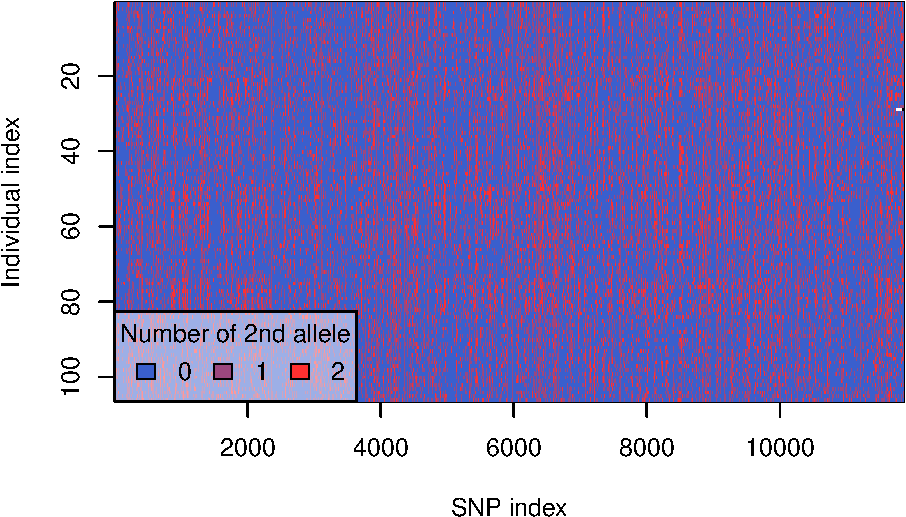
\includegraphics{Final-Report_files/figure-latex/unnamed-chunk-5-1.pdf}

The log-log plot shows an approximately linear relationship between the
natural log of the variance and the natural log of the mean.

\begin{verbatim}
## [1] "After filtering, the number of genes remaining in the dataset are: 2470"
\end{verbatim}

Finally, the data was split into training and test sets. The ratio was
80\% training and 20\% test set with each population split evenly among
the two sets.

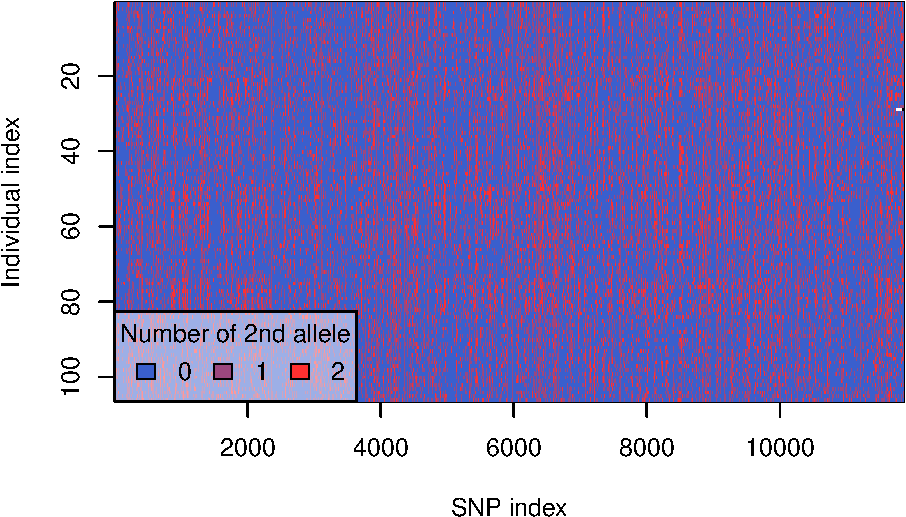
\includegraphics{Final-Report_files/figure-latex/unnamed-chunk-9-1.pdf}

\begin{Shaded}
\begin{Highlighting}[]
\CommentTok{\#Create frequency plot with symmetry}
\NormalTok{myFreq }\OtherTok{\textless{}{-}} \FunctionTok{glMean}\NormalTok{(x)}
\NormalTok{myFreq }\OtherTok{\textless{}{-}} \FunctionTok{c}\NormalTok{(myFreq, }\DecValTok{1}\SpecialCharTok{{-}}\NormalTok{myFreq)}
\FunctionTok{hist}\NormalTok{(myFreq, }\AttributeTok{proba=}\ConstantTok{TRUE}\NormalTok{, }\AttributeTok{col=}\StringTok{"darkseagreen3"}\NormalTok{, }\AttributeTok{xlab=}\StringTok{"Allele frequencies"}\NormalTok{,}
\AttributeTok{main=}\StringTok{"Distribution of allele frequencies"}\NormalTok{, }\AttributeTok{nclass=}\DecValTok{20}\NormalTok{, }\AttributeTok{ylim =} \FunctionTok{c}\NormalTok{(}\DecValTok{0}\NormalTok{,}\FloatTok{3.5}\NormalTok{))}
\NormalTok{temp }\OtherTok{\textless{}{-}} \FunctionTok{density}\NormalTok{(myFreq, }\AttributeTok{bw=}\NormalTok{.}\DecValTok{05}\NormalTok{)}
\FunctionTok{lines}\NormalTok{(temp}\SpecialCharTok{$}\NormalTok{x, temp}\SpecialCharTok{$}\NormalTok{y}\SpecialCharTok{*}\DecValTok{2}\NormalTok{,}\AttributeTok{lwd=}\DecValTok{3}\NormalTok{)}
\end{Highlighting}
\end{Shaded}

\includegraphics{Final-Report_files/figure-latex/unnamed-chunk-10-1.pdf}

\begin{Shaded}
\begin{Highlighting}[]
\CommentTok{\# An empty plot.}
\CommentTok{\#freq\_peak\_plot(pos=1:40)}
\NormalTok{gt }\OtherTok{\textless{}{-}} \FunctionTok{extract.gt}\NormalTok{(vcf)}
\NormalTok{hets }\OtherTok{\textless{}{-}} \FunctionTok{is\_het}\NormalTok{(gt)}
\CommentTok{\# Censor non{-}heterozygous positions.}
\FunctionTok{is.na}\NormalTok{(vcf}\SpecialCharTok{@}\NormalTok{gt[,}\SpecialCharTok{{-}}\DecValTok{1}\NormalTok{][}\SpecialCharTok{!}\NormalTok{hets]) }\OtherTok{\textless{}{-}} \ConstantTok{TRUE}
\CommentTok{\# Extract allele depths.}
\NormalTok{ad }\OtherTok{\textless{}{-}} \FunctionTok{extract.gt}\NormalTok{(vcf, }\AttributeTok{element =} \StringTok{"AD"}\NormalTok{)}
\NormalTok{ad1 }\OtherTok{\textless{}{-}} \FunctionTok{masplit}\NormalTok{(ad, }\AttributeTok{record =} \DecValTok{1}\NormalTok{)}
\NormalTok{ad2 }\OtherTok{\textless{}{-}} \FunctionTok{masplit}\NormalTok{(ad, }\AttributeTok{record =} \DecValTok{2}\NormalTok{)}
\NormalTok{freq1 }\OtherTok{\textless{}{-}}\NormalTok{ ad1}\SpecialCharTok{/}\NormalTok{(ad1}\SpecialCharTok{+}\NormalTok{ad2)}
\NormalTok{freq2 }\OtherTok{\textless{}{-}}\NormalTok{ ad2}\SpecialCharTok{/}\NormalTok{(ad1}\SpecialCharTok{+}\NormalTok{ad2)}
\NormalTok{myPeaks1 }\OtherTok{\textless{}{-}} \FunctionTok{freq\_peak}\NormalTok{(freq1, }\FunctionTok{getPOS}\NormalTok{(vcf))}
\FunctionTok{is.na}\NormalTok{(myPeaks1}\SpecialCharTok{$}\NormalTok{peaks[myPeaks1}\SpecialCharTok{$}\NormalTok{counts }\SpecialCharTok{\textless{}} \DecValTok{20}\NormalTok{]) }\OtherTok{\textless{}{-}} \ConstantTok{TRUE}
\NormalTok{myPeaks2 }\OtherTok{\textless{}{-}} \FunctionTok{freq\_peak}\NormalTok{(freq2, }\FunctionTok{getPOS}\NormalTok{(vcf), }\AttributeTok{lhs =} \ConstantTok{FALSE}\NormalTok{)}
\FunctionTok{is.na}\NormalTok{(myPeaks2}\SpecialCharTok{$}\NormalTok{peaks[myPeaks2}\SpecialCharTok{$}\NormalTok{counts }\SpecialCharTok{\textless{}} \DecValTok{20}\NormalTok{]) }\OtherTok{\textless{}{-}} \ConstantTok{TRUE}
\FunctionTok{freq\_peak\_plot}\NormalTok{(}\AttributeTok{pos =} \FunctionTok{getPOS}\NormalTok{(vcf), }\AttributeTok{ab1 =}\NormalTok{ freq1, }\AttributeTok{ab2 =}\NormalTok{ freq2, }\AttributeTok{fp1 =}\NormalTok{ myPeaks1, }\AttributeTok{fp2=}\NormalTok{myPeaks2)}
\end{Highlighting}
\end{Shaded}

\includegraphics{Final-Report_files/figure-latex/unnamed-chunk-11-1.pdf}

\section{Models}\label{models}

\subsection{Data Pre-Processing}\label{data-pre-processing}

\subsection{Algorithm Selection}\label{algorithm-selection}

My proposed analysis will be to use at least two different types of
Machine Learning Analysis, including one random forest model and one
Support Vector Machine. Depending on the outcome of those models, deep
neural networks have also been demonstrated to be effective when working
with genetic data (Elgart et al., 2022). The Random Forest algorithm was
chosen for its robustness and ability to handle high-dimensional data,
making it suitable for gene expression analysis. I also plan to use gini
importance to attempt to identify SNPs that may be the most important
for differences between cultivars in this dataset. SVMs are also capable
of working with non-linear data. Appropriate feature selection and
dimensionality reduction measures will probably be necessary. The nature
of the available environmental and geographical data may influence the
efficacy of the analysis. The analysis will predict which SNPs indicate
cultivar differences due to environmental factors. The hypothesis can be
supported if the predictive model trained on the data can accurately
identify the same SNPs on unseen data.

\subsection{Final Model}\label{final-model}

\section{Conclusions}\label{conclusions}

In order to access and manipulate the VCF file, several additional R
packages were used. The vcfR package allows for loading and manipulation
of the data, while the adegenet package was helpful in creating several
of the visualizations.

\section{Discussion and Next Steps}\label{discussion-and-next-steps}

\section{Code Availability}\label{code-availability}

The code used for this research is available at:
\url{https://github.com/samanthaharper/sassafras_capstone}

The code is available within the rmd version of this report or in the
final code R file.

\section{References}\label{references}

Elgart, M., Lyons, G., Romero-Brufau, S. et al.~Non-linear machine
learning models incorporating SNPs and PRS improve polygenic prediction
in diverse human populations. Commun Biol 5, 856 (2022).
\url{https://doi.org/10.1038/s42003-022-03812-z} Guan, B., Liu, Q., Liu,
X. et al.~Environment influences the genetic structure and genetic
differentiation of Sassafras tzumu (Lauraceae). BMC Ecol Evo 24, 80
(2024). \url{https://doi.org/10.1186/s12862-024-02264-9} Silva, P.P.,
Gaudillo, J.D., Vilela, J.A. et al.~A machine learning-based SNP-set
analysis approach for identifying disease-associated susceptibility
loci. Sci Rep 12, 15817 (2022).
\url{https://doi.org/10.1038/s41598-022-19708-1} Zhang K, Zhang Y, Jia
D, Tao J. Species Distribution Modeling of Sassafras Tzumu and
Implications for Forest Management. Sustainability. 2020; 12(10):4132.
\url{https://doi.org/10.3390/su12104132}

\end{document}
